\documentclass[10pt]{article}

%This is the minimal setup required to render the flag
\usepackage[paperwidth=144cm, paperheight=96cm, top=0cm, bottom=0cm, left=0cm, right=0cm]{geometry}
%Paper width is set to 144cm by 96cm to match the ROK Government-specified aspect ratio (3:2)
\usepackage{tikz}
%\usepackage[dvipsnames]{xcolor} % Optional unless you want to use colors pre-defined by the xcolor package

% ROK Government-specified colors for the flag
\definecolor{rokred}{HTML}{CD2E3A}
\definecolor{rokblue}{HTML}{0047A0}
\definecolor{rokwhite}{HTML}{FFFFFF}
\definecolor{rokblack}{HTML}{000000}

% Other government specifications include:
% Taegeuk (central circle) diameter is 1/3 flag width, here it is 48cm
% Each block of bars has width 1/9 flag width (here it is 16cm) and height 1/6 flag width (here it is 24cm)
% Spacing between bars within each block (vertical or horizontal) is 1/72 flag width, here it is 2cm
% Shortest distance from edge of Taegeuk to edge of each block of bars is 1/12 flag width, here it is 12cm

%Source: https://commons.wikimedia.org/wiki/File:Flag_of_South_Korea_(construction_sheet).svg

%Created by Senan Sekhon, August 5, 2021

\begin{document}

\begin{center} %Optional, but helps to tidy up the layout
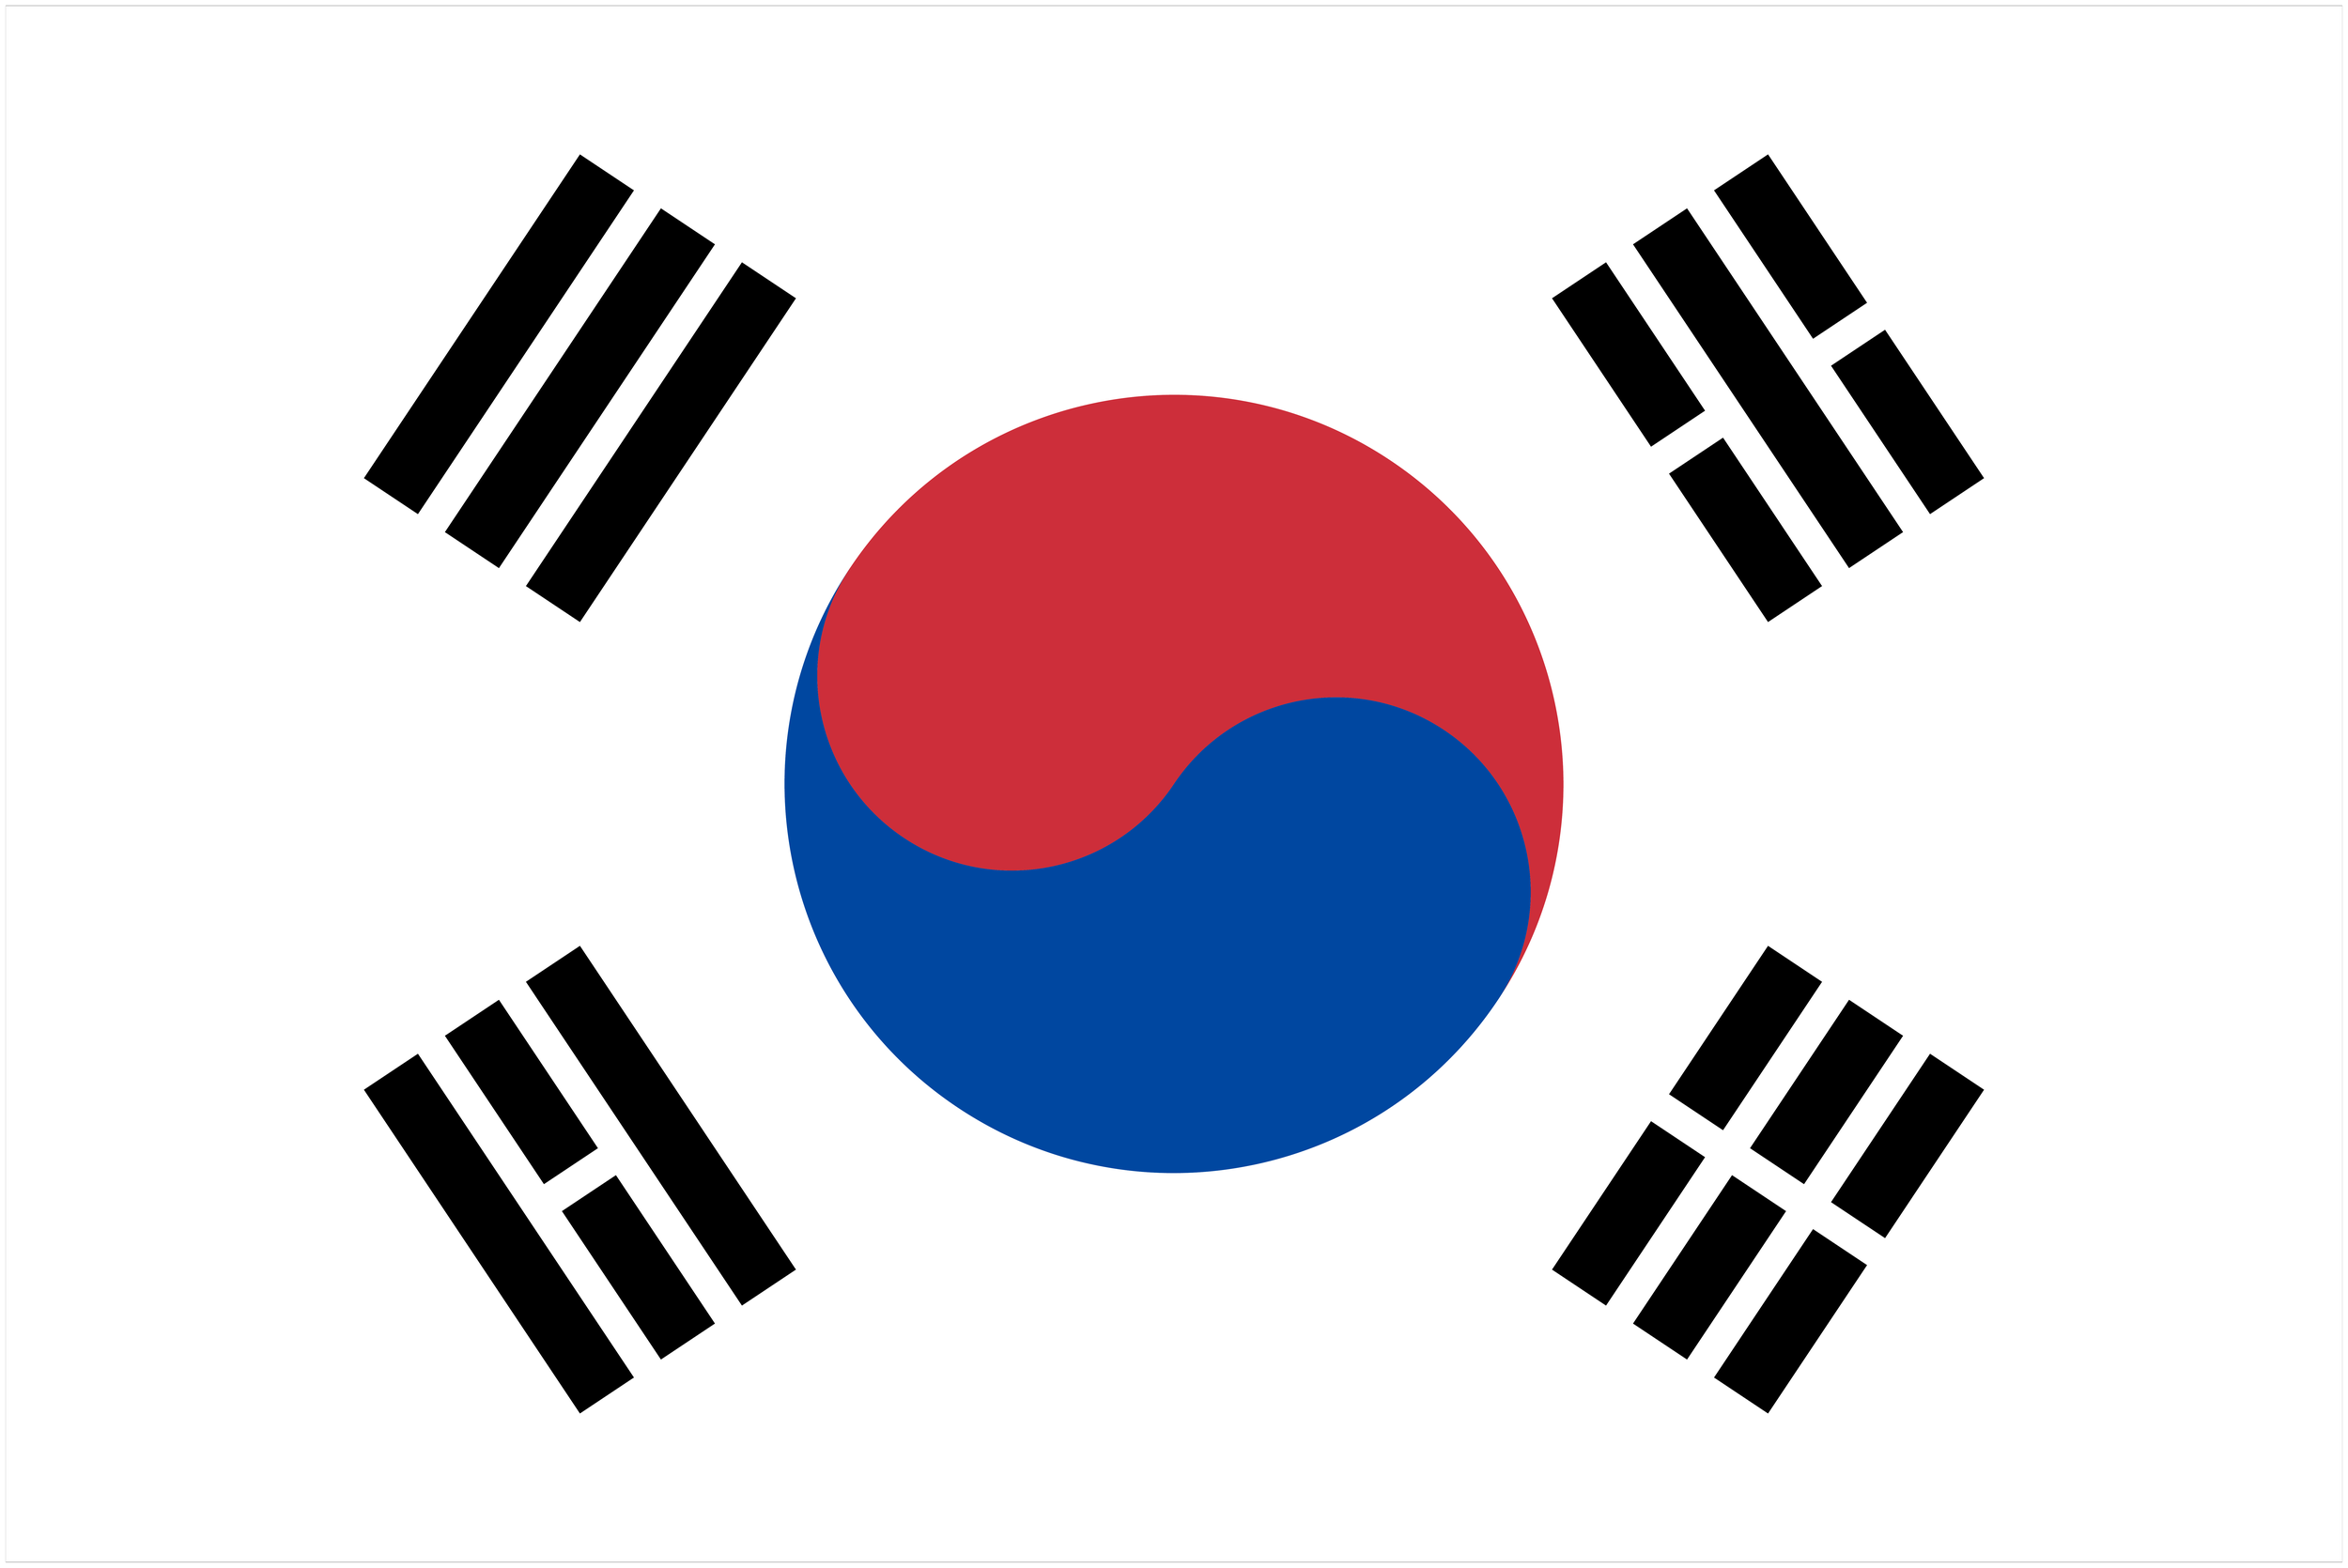
\begin{tikzpicture}[scale=1] %Scale must be changed to make the flag fit on letter/A4 paper (scale=1 produces a 144cm by 96cm flag)
\clip (-72,-48) rectangle (72,48); %Optional, crops the flag to the correct size
\draw[-] (-72,-48) rectangle (72,48); %Optional, draws a border around the flag
\fill[rokred] (0,0) arc({-atan(2/3)}:{-180-atan(2/3)}:12) arc({180-atan(2/3)}:{-atan(2/3)}:24) arc({-atan(2/3)}:{180-atan(2/3)}:12); %Taegeuk top half (red)
\fill[rokblue] (0,0) arc({180-atan(2/3)}:{-atan(2/3)}:12) arc({-atan(2/3)}:{-180-atan(2/3)}:24) arc({180-atan(2/3)}:{360-atan(2/3)}:12); %Taegeuk bottom half (blue)
\begin{scope}[shift={({-132/sqrt(13)},{88/sqrt(13)})},rotate=-atan(2/3)] %Top-left block (3 bars)
\fill[rokblack] (-8,-12) rectangle (-4,12);
\fill[rokblack] (-2,-12) rectangle (2,12);
\fill[rokblack] (4,-12) rectangle (8,12);
\end{scope}
\begin{scope}[shift={({132/sqrt(13)},{88/sqrt(13)})},rotate=atan(2/3)] %Top-right block (5 bars)
\fill[rokblack] (-8,-12) rectangle (-4,-1);
\fill[rokblack] (-8,1) rectangle (-4,12);
\fill[rokblack] (-2,-12) rectangle (2,12);
\fill[rokblack] (4,-12) rectangle (8,-1);
\fill[rokblack] (4,1) rectangle (8,12);
\end{scope}
\begin{scope}[shift={({-132/sqrt(13)},{-88/sqrt(13)})},rotate=atan(2/3)] %Bottom-left block (4 bars)
\fill[rokblack] (-8,-12) rectangle (-4,12);
\fill[rokblack] (-2,-12) rectangle (2,-1);
\fill[rokblack] (-2,1) rectangle (2,12);
\fill[rokblack] (4,-12) rectangle (8,12);
\end{scope}
\begin{scope}[shift={({132/sqrt(13)},{-88/sqrt(13)})},rotate=-atan(2/3)] %Bottom-right block (6 bars)
\fill[rokblack] (-8,-12) rectangle (-4,-1);
\fill[rokblack] (-8,1) rectangle (-4,12);
\fill[rokblack] (-2,-12) rectangle (2,-1);
\fill[rokblack] (-2,1) rectangle (2,12);
\fill[rokblack] (4,-12) rectangle (8,-1);
\fill[rokblack] (4,1) rectangle (8,12);
\end{scope}
\end{tikzpicture}
\end{center}

\end{document}